% Trecho autônomo para leitura. Integração no TCC: ver README.md.
% Aparência reconstruída a partir do PDF da proposta do autor; não é classe oficial.
\documentclass[12pt,a4paper,oneside]{article}
\usepackage[T1]{fontenc}
\usepackage[utf8]{inputenc}
\usepackage[brazil]{babel}
\usepackage[left=3cm,top=3cm,right=2cm,bottom=2cm]{geometry}
\usepackage{lmodern,microtype,indentfirst}
\usepackage{graphicx,booktabs,longtable,amsmath,array,setspace,tabularx}
\usepackage{fancyhdr,caption,pdflscape,placeins}
\usepackage[authoryear,round]{natbib}
\usepackage[hidelinks]{hyperref}
\hypersetup{pdftitle={Metodologia e resultados da coorte ampliada de letras},pdfauthor={Felipe Macedo Cordeiro}}
\onehalfspacing
\setlength{\parindent}{1.25cm}
\setlength{\parskip}{0pt}
\setlength{\headheight}{16pt}
\setlength{\emergencystretch}{2em}
\pagestyle{fancy}
\fancyhf{}
\fancyhead[L]{\small\itshape\nouppercase{\leftmark}}
\fancyhead[R]{\small\thepage}
\renewcommand{\sectionmark}[1]{\markboth{#1}{}}
\renewcommand{\headrulewidth}{0.4pt}
\captionsetup{font=small,labelfont=bf}
\newcommand{\fonte}[1]{\par\smallskip{\footnotesize Fonte: #1\par}}
\newcommand{\nota}[1]{\par\smallskip{\footnotesize Nota: #1\par}}
\newcolumntype{Y}{>{\raggedright\arraybackslash}X}
\numberwithin{equation}{subsection}
\setcounter{section}{2}
\begin{document}
\section{Metodologia da análise da coorte ampliada}
\label{sec:metodologia}

O objetivo desta etapa foi avaliar se descritores de letras acrescentam informação para estimar a popularidade Spotify registrada na base, além daquela disponível em características acústicas e metadados. A questão não consiste em identificar uma fórmula de sucesso comercial, mas em comparar a capacidade preditiva de dois conjuntos de variáveis sob as mesmas condições de avaliação. Foram comparados o bloco \textit{Baseline}, com 23 atributos, e o bloco \textit{Tradicional}, com os mesmos 23 atributos acrescidos de 196 descritores de letras.

A análise foi implementada em Python e realizada exclusivamente no conjunto de desenvolvimento. As previsões avaliadas foram produzidas para observações que não participaram do ajuste do respectivo modelo. O conjunto de teste originalmente reservado não foi utilizado para escolher transformações, hiperparâmetros ou famílias de regressão nesta rodada. Como esta etapa ocorreu após análises anteriores do estudo, seus resultados têm caráter exploratório.

\subsection{Adequações em relação à proposta inicial}

A proposta inicial previa obtenção de dados pelas APIs do Spotify e do Genius, restrição a músicas em inglês, implementação em R e amostragem com quantidades iguais em estratos de popularidade. A execução aqui descrita adotou um desenho diferente: reutilizou a base integrada Spotify--LFM2b, os descritores já disponíveis e as letras aceitas na coleta do LRCLIB, com implementação em Python. A presente auditoria de integridade não estabeleceu que todas as letras fossem em inglês; por isso, essa restrição não é apresentada como característica comprovada da coorte.

Outra diferença fundamental é que não foram selecionadas quantidades iguais de músicas em cada faixa de popularidade. Utilizou-se a coorte elegível com letras aceitas, respeitando a divisão de desenvolvimento e teste já existente. Consequentemente, o número de composições de alta popularidade corresponde à disponibilidade nessa coorte, e não a uma cota previamente preenchida. O balanceamento previsto na proposta original não deve ser descrito como procedimento executado.

Também foi delimitada a interpretação do desfecho. A resposta analisada é a popularidade observada no momento de referência da fonte, denominado \textit{snapshot}. Não se trata de uma observação futura feita após o treinamento, nem de uma medida direta de lucro, vendas ou sucesso comercial. Essa distinção é necessária para que a conclusão corresponda ao que os dados permitem avaliar.

\subsection{Formação da amostra e unidade de análise}

A coleta e a auditoria identificaram 78.323 faixas com letras aceitas, sendo 58.705 vinculadas ao desenvolvimento e 19.618 ao teste reservado. Esses números descrevem faixas, isto é, registros associados a identificadores de gravações. Eles não correspondem necessariamente ao número de composições musicais distintas.

Uma mesma composição pode aparecer em mais de uma versão. Para reduzir sua repetição na análise, selecionou-se um representante por chave operacional de composição dentro do subconjunto aceito. A escolha foi determinística e não utilizou popularidade: considerou critérios já implementados de versão, confiança do pareamento, completude e desempate por identificadores. Foram colapsadas 72 versões adicionais no desenvolvimento, resultando em \textbf{58.633 composições operacionais}. Os vínculos das demais faixas foram preservados para rastreabilidade.

A expressão composição operacional indica uma identificação construída a partir das regras do projeto; não equivale a um identificador universal de uma obra musical. Cada linha da matriz representa uma dessas composições por meio de uma faixa selecionada. A Tabela~\ref{tab:amostra} distingue as etapas e evita confundir o universo coletado com o tamanho efetivamente usado na modelagem.

\begin{table}[htbp]
\centering\small
\caption{Da coleção aceita à matriz de desenvolvimento}\label{tab:amostra}
\begin{tabularx}{\textwidth}{Yr}
\toprule Etapa ou unidade & Quantidade\\\midrule
Faixas com letras aceitas nos dois conjuntos & 78.323\\
Faixas aceitas no desenvolvimento & 58.705\\
Faixas aceitas no teste reservado & 19.618\\
Versões adicionais colapsadas no desenvolvimento & 72\\
Composições operacionais usadas nesta rodada & 58.633\\
Grupos de artista na matriz de desenvolvimento & 8.883\\
Componentes de dependência utilizados na validação & 8.880\\
\bottomrule
\end{tabularx}
\fonte{Registros de preparação e descrição da coorte aceita, execução de outubro de 2026.}
\end{table}

A auditoria encontrou 78.280 textos distintos por hash entre as 78.323 consultas aceitas. Um hash é uma assinatura computacional do texto: permite detectar igualdade exata, mas não demonstra que duas versões diferentes sejam semanticamente equivalentes. A contagem de textos distintos é diferente da contagem de composições. Textos repetidos foram considerados na construção dos grupos de validação, sem exclusão automática de composições apenas por compartilharem letra.

\subsection{Variável resposta e blocos de preditoras}

A variável resposta, denotada por $Y$, é o índice \texttt{spotify\_popularity}, cuja escala nominal vai de 0 a 100. Na coorte analisada, o intervalo efetivamente observado foi de 0 a 85. Um valor 80 não significa que 80\% das pessoas conheçam a música; trata-se da pontuação registrada na fonte.

O bloco Baseline reuniu características acústicas, duração, ano, gênero e indicadores de versão. Os 23 campos autorizados foram \texttt{year}, \texttt{genre}, \texttt{danceability}, \texttt{energy}, \texttt{key}, \texttt{loudness}, \texttt{mode}, \texttt{speechiness}, \texttt{acousticness}, \texttt{instrumentalness}, \texttt{liveness}, \texttt{valence}, \texttt{tempo}, \texttt{duration\_ms}, \texttt{time\_signature}, \texttt{remaster}, \texttt{remix}, \texttt{live}, \texttt{acoustic}, \texttt{radio\_edit}, \texttt{mono\_stereo}, \texttt{instrumental} e \texttt{demo}. Ano e gênero mantiveram a semântica documentada para a fonte, sem atribuir ao ano, por exemplo, uma interpretação universal de primeira publicação da composição.

O bloco Tradicional acrescentou 196 descritores LFM2b autorizados no manifesto do projeto. Esses descritores quantificam propriedades lexicais, de diversidade, legibilidade, rima, estrutura e conteúdo afetivo. Logo, esse bloco utiliza informação sobre letras, mas não corresponde a uma nova rede neural lendo os textos completos. Os descritores foram reaproveitados, sem recálculo a partir das letras LRCLIB. A possível diferença entre a versão textual de origem do descritor e a letra posteriormente recuperada permanece uma limitação.

O Tradicional possui, portanto, 219 atributos de entrada antes da codificação de categorias e da expansão por splines. Esse número não é necessariamente igual ao número de coeficientes ajustados. Ambos os blocos utilizaram as mesmas 58.633 observações. Artista, título, identificadores, informações do pareamento, status de coleta, visualizações no Genius e contagens de reprodução no LFM não foram utilizados como preditores. A popularidade ficou exclusivamente no vetor resposta, separado da matriz de entrada.

\subsection{Descrição e preparação dos dados}

Foram examinadas a distribuição empírica da resposta, suas frequências, quantis, média e dispersão, além das ausências e associações entre variáveis. A descrição antecedeu a modelagem e não foi usada para excluir observações por popularidade ou por dificuldade de previsão. Encontraram-se 233 pares de preditoras com correlação de Spearman em valor absoluto de pelo menos 0,8, considerando pares completos. Essa redundância motivou a comparação de regressões com regularização, sem justificar a remoção automática de variáveis.

Oito descritores estruturais apresentaram 23.699 ausências cada um, aproximadamente 40,4\% das 58.633 observações. As ausências numéricas foram tratadas pela mediana calculada no respectivo treinamento, seguida de padronização das variáveis numéricas também com parâmetros do treino. Nenhuma dessas estatísticas foi estimada usando as observações externas de validação. Para colunas inteiramente ausentes em um treino, o procedimento preserva a coluna com preenchimento por zero.

Gênero, tonalidade e assinatura de compasso foram tratados como categorias, sem impor uma distância numérica ordinal à tonalidade. As categorias foram codificadas por indicadores, omitindo-se uma categoria de referência. Categorias ausentes receberam marcador explícito; categorias não vistas no treino receberam o vetor de indicadores nulo. Modalidade e indicadores de versão foram tratados como binários.

Nos modelos regularizados do Tradicional, compararam-se descritores originais com a transformação $\operatorname{asinh}(x)$, que comprime valores extremos de forma monotônica e admite zeros e números negativos. A escolha ocorreu na validação interna. Essa transformação não apagou registros, não retirou variáveis e não alterou os dados originais. Não foi aplicada análise de componentes principais nesta rodada.

\subsection{Famílias de regressão comparadas}

Os nomes Baseline e Tradicional designam conjuntos de atributos, e não algoritmos. Cada conjunto foi analisado com quatro famílias de regressão. A comparação permite distinguir a contribuição da forma do modelo da contribuição das informações textuais. Regressão, regularização e modelos aditivos integram a abordagem estatística de aprendizagem supervisionada discutida por \citet{james2023}.

Na regressão linear por mínimos quadrados ordinários, ou MQO, a média condicional é representada por uma combinação linear dos atributos:
\begin{equation}
\widehat{Y}_i=\widehat{\beta}_0+\sum_{j=1}^{p}\widehat{\beta}_j X_{ij}.
\end{equation}
Os coeficientes são escolhidos para reduzir a soma dos erros quadráticos no treinamento. A forma linear é uma hipótese sobre a relação entre os atributos e a resposta; ela não exige que o histograma marginal da popularidade seja normal para que o ajuste seja realizado.

A regressão Ridge também utiliza uma combinação linear, mas penaliza coeficientes muito grandes. Essa penalização pode estabilizar o ajuste quando variáveis carregam informações semelhantes. O Elastic Net combina duas formas de penalização e pode reduzir alguns coeficientes a zero. Portanto, Elastic Net já é uma regressão linear regularizada, e não uma alternativa conceitualmente oposta à regressão.

A regressão aditiva com Ridge permite que determinadas variáveis contínuas apresentem relações curvas com a resposta. Em vez de exigir uma única reta para o ano ou a dançabilidade, por exemplo, o modelo combina funções suaves, representadas por splines:
\begin{equation}
\widehat{Y}_i=\widehat{\beta}_0+\sum_{j\in\mathcal{S}}\widehat{f}_j(X_{ij})+
\sum_{j\notin\mathcal{S}}\widehat{\beta}_jX_{ij}.
\end{equation}
O conjunto $\mathcal{S}$ incluiu ano, dançabilidade, energia, intensidade sonora, presença de fala, acusticidade, instrumentalidade, presença de público, valência, andamento e duração. Foram usadas bases cúbicas com cinco nós uniformes por variável, aprendidos no treino, e extrapolação linear. O ajuste é aditivo: não inclui automaticamente todas as interações entre variáveis. Trata-se de regressão em bases spline com penalização Ridge, não de uma rede neural nem de um GAM ajustado por REML.

Para Ridge e para a regressão aditiva, compararam-se valores de penalização iguais a 1, 100 e 1.000. Para Elastic Net, foram considerados $\alpha\in\{0{,}03;0{,}3\}$ e proporção L1 em $\{0{,}1;0{,}8\}$. A comparação entre descritores originais e transformados duplicou as configurações desses métodos no Tradicional. A grade foi estabelecida antes dos ajustes e não foi ampliada para favorecer os resultados. Conclusões sobre superioridade dizem respeito a essas configurações, não a todas as versões possíveis dos algoritmos.

Também foram ajustadas duas referências constantes: uma prevê a média e outra a mediana da popularidade do treino para qualquer composição. Elas mostram o erro obtido sem utilizar características das músicas e ajudam a interpretar se os modelos acrescentam capacidade preditiva.

\subsection{Validação agrupada e significado do tamanho utilizado}

Registros relacionados não foram distribuídos livremente entre treino e validação. Foram construídos componentes que reúnem qualquer vínculo conhecido de artista, composição, grupo original de split ou texto idêntico. As relações são transitivas: se duas faixas estão ligadas por artista e uma delas compartilha texto com uma terceira, as três pertencem ao mesmo componente. Isso resultou em 8.880 componentes de validação, ligeiramente menos que os 8.883 grupos de artista. O maior componente continha 256 composições.

Esses componentes foram divididos em cinco partes externas, denominadas \textit{folds}. Em cada rodada, quatro partes serviram ao treinamento e uma ficou reservada para avaliação. Cada composição recebeu uma previsão externa uma única vez. Ao reunir essas previsões, obteve-se o conjunto \textit{out-of-fold} (OOF) de 58.633 observações. Os tamanhos de cada rodada estão na Tabela~\ref{tab:folds}.

\begin{table}[htbp]
\centering\small
\caption{Tamanhos dos treinamentos e validações externas}\label{tab:folds}
\begin{tabular}{crr}
\toprule
Fold & Treinamento & Validação externa\\\midrule
1 & 47.016 & 11.617\\
2 & 46.555 & 12.078\\
3 & 46.959 & 11.674\\
4 & 47.170 & 11.463\\
5 & 46.832 & 11.801\\
\bottomrule
\end{tabular}
\fonte{Elaboração a partir dos resultados salvos da coorte aceita.}
\nota{As cinco validações somam 58.633 observações distintas. O benchmark de 3.008 linhas foi apenas um teste técnico.}
\end{table}


Assim, nenhum ajuste externo utilizou as 58.633 linhas simultaneamente como treino: cada um aprendeu com aproximadamente 46,6 a 47,2 mil composições e foi avaliado em aproximadamente 11,5 a 12,1 mil. A divisão externa em cinco folds ocorreu dentro do desenvolvimento e não substituiu o split original de 75\%/25\%. Os alvos das faixas do holdout permaneceram fora dessa avaliação.

Dentro de cada treinamento externo, foram criadas três partes internas, respeitando os mesmos componentes. As configurações foram escolhidas pela média do MAE nessas três validações internas. Somente depois da escolha foi ajustado o modelo no treino externo completo e prevista sua validação externa. Essa separação reduz o viés de avaliar um modelo nos mesmos dados usados para escolhê-lo, problema discutido por \citet{cawley2010}.

Em termos práticos, esconder a resposta da validação significa não fornecê-la ao modelo no momento da previsão. Não significa substituí-la por zero, modificar a base ou deixar de usá-la posteriormente para medir o erro. Para cada previsão OOF, a resposta correspondente só participa da comparação entre valor previsto e observado.

O benchmark inicial utilizou 3.008 observações para verificar custo e funcionamento. Esse lote não foi a amostra final de treinamento. A execução completa realizou 480 ajustes internos e 50 externos, além dos oito ajustes técnicos do benchmark. Os 50 modelos externos correspondem a quatro famílias, dois blocos e cinco folds, mais duas referências constantes em cinco folds. A repetição de ajustes não cria novas observações independentes.

\subsection{Métricas e avaliação da contribuição incremental}

Se $y_i$ é a popularidade observada e $\widehat{y}_i$ sua previsão OOF, o erro absoluto médio e a raiz do erro quadrático médio são definidos por:
\begin{align}
\operatorname{MAE}&=\frac{1}{n}\sum_{i=1}^{n}|y_i-\widehat{y}_i|,\\
\operatorname{RMSE}&=\sqrt{\frac{1}{n}\sum_{i=1}^{n}(y_i-\widehat{y}_i)^2}.
\end{align}
Ambas são expressas em pontos da escala de popularidade. Como exemplo exclusivamente ilustrativo, uma música observada com 20 pontos e prevista com 26 produz erro absoluto de 6 pontos. O MAE resume a média desses erros; o RMSE atribui maior peso aos erros grandes. Um MAE de 6,89 não significa erro máximo de 6,89, nem 93,11\% de acerto.

O coeficiente de determinação foi calculado no conjunto OOF por:
\begin{equation}
R^2=1-\frac{\sum_i(y_i-\widehat{y}_i)^2}{\sum_i(y_i-\overline{y})^2}.
\end{equation}
Um $R^2$ de 0,56 indica que o erro quadrático agregado corresponde a aproximadamente 44\% da variação quadrática em torno da média observada usada nessa definição. Não significa que 56\% das músicas foram previstas corretamente. A média no denominador é uma referência matemática de avaliação; não foi fornecida ao modelo como informação da validação.

Foram calculados ainda mediana, percentis 90 e 95 do erro absoluto, frequência de erros superiores a 20 pontos e previsões fora de 0--100. O percentil 95, ou P95, informa o valor abaixo do qual se encontram aproximadamente 95\% dos erros observados; não é um intervalo individual de previsão. As previsões foram mantidas sem corte nos limites da escala.

A contribuição dos descritores foi avaliada por diferenças Tradicional menos Baseline, dentro da mesma família e nas mesmas observações. Para erros, diferenças negativas favorecem o Tradicional. Intervalos exploratórios de 95\% foram obtidos por 1.000 reamostragens pareadas de componentes completos, mantendo fixas as previsões OOF. Esses intervalos não incorporam toda a variação de repetir treinamento e seleção, e os cinco folds não são tratados como cinco experimentos independentes.

\clearpage
\section{Resultados da modelagem na coorte aceita}
\label{sec:resultados}

\subsection{Distribuição da popularidade e presença de valores elevados}

A popularidade das 58.633 composições apresentou média de 26,01 pontos, mediana de 25 e desvio-padrão de 13,44. Metade das observações estava entre 16 e 34 pontos; o percentil 95 foi 51 e o percentil 99 foi 62. O máximo observado foi 85, e 246 composições tinham valor zero. Esses números mostram que a maior parte da coorte está concentrada nas regiões baixa e intermediária da escala, com uma cauda à direita.

\begin{table}[htbp]
\centering\small
\caption{Distribuição das composições por faixa de popularidade}\label{tab:distribuicao}
\begin{tabular}{lrr}
\toprule
Popularidade & Composições & Participação (\%)\\\midrule
0 a 9 & 5.694 & 9,711\\
10 a 19 & 14.822 & 25,279\\
20 a 29 & 16.747 & 28,562\\
30 a 39 & 12.138 & 20,702\\
40 a 49 & 5.799 & 9,890\\
50 a 59 & 2.512 & 4,284\\
60 a 69 & 772 & 1,317\\
70 a 79 & 138 & 0,235\\
80 a 89 & 11 & 0,019\\
90 a 100 & 0 & 0,000\\
Total & 58.633 & 100,000\\
\bottomrule
\end{tabular}
\fonte{Elaboração a partir dos resultados salvos da coorte aceita.}
\nota{As faixas referem-se à resposta observada; não foram usadas para excluir observações. Percentuais arredondados podem não somar exatamente 100.}
\end{table}


\textbf{As 11 observações mencionadas na análise correspondem somente às composições com popularidade entre 80 e 89 pontos.} Elas representam aproximadamente 0,019\% da amostra de desenvolvimento. Não são as únicas músicas consideradas populares em qualquer sentido: havia também 138 composições entre 70 e 79 e 772 entre 60 e 69. Ao considerar valores iguais ou superiores a 70, o total é 149; com limiar de 60, são 921. Não houve observação de 90 a 100 nessa matriz. Esses limiares são faixas descritivas, não categorias universais de sucesso.

O número pequeno não resulta de treinamento feito com apenas 11 músicas, nem de exclusão das que o modelo errou. Todas as 58.633 composições foram incluídas na avaliação OOF. A contagem de 11 decorre da distribuição da resposta na coorte resultante da integração, da disponibilidade de letras aceitas, do split preservado e da seleção de representantes. Como não houve amostragem com cotas iguais de popularidade, não se garantiu um número mínimo de casos na cauda.

Não é possível atribuir esse desequilíbrio a uma única causa com os resumos disponíveis. Há, porém, evidência descritiva de cobertura desigual: no nível de faixa do desenvolvimento, as 58.705 faixas com letras aceitas apresentaram popularidade média de 26,01, enquanto as 25.112 sem letra aceita tiveram média de 29,76. Isso indica que condicionar a análise à disponibilidade de letra modifica o perfil observado. Não demonstra que a obtenção de letra cause menor popularidade, nem que o LRCLIB seja a única origem da diferença.

Consequentemente, a amostra não deve ser descrita como retrato representativo de todas as músicas do Spotify. Ter muitas observações reduz algumas fontes de instabilidade, mas não corrige automaticamente seleção da base ou escassez em determinadas regiões da resposta. A Figura~\ref{fig:distribuicao} apresenta a distribuição empírica; o gráfico QQ marginal não constitui teste dos pressupostos dos resíduos de uma regressão.

\begin{figure}[htbp]
\centering
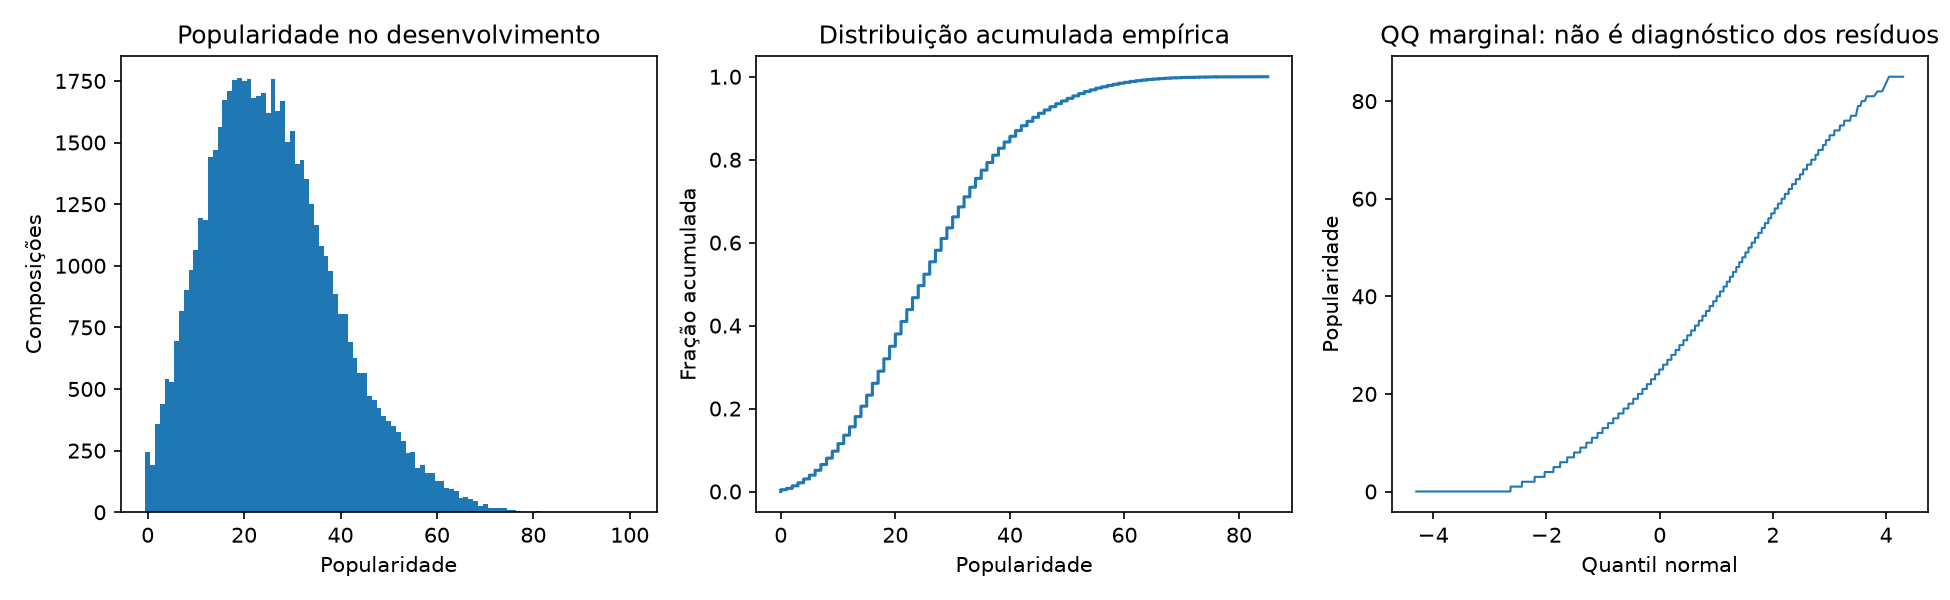
\includegraphics[width=\textwidth]{images/distribuicao_popularidade.png}
\caption{Distribuição, frequência acumulada e gráfico QQ marginal da popularidade no desenvolvimento}\label{fig:distribuicao}
\fonte{Análise descritiva da coorte aceita. Figura original preservada.}
\end{figure}

\subsection{Comparação das famílias de regressão}

A Tabela~\ref{tab:modelos} apresenta os resultados globais de validação cruzada. Todas as linhas foram avaliadas sobre as mesmas 58.633 composições, permitindo comparação direta dentro desta rodada. Não se trata de comparar erros de treinamento.

\begin{table}[htbp]
\centering\small
\caption{Desempenho OOF das famílias de regressão}\label{tab:modelos}
\begin{tabular}{llrrr}
\toprule
Família & Bloco & MAE & RMSE & $R^2$\\\midrule
Linear comum & Baseline & 7,0536 & 9,1360 & 0,5378\\
Linear comum & Tradicional & 6,9854 & 9,0549 & 0,5460\\
Ridge & Baseline & 7,0524 & 9,1340 & 0,5380\\
Ridge & Tradicional & 6,9712 & 9,0269 & 0,5488\\
Elastic Net & Baseline & 7,4490 & 9,6340 & 0,4860\\
Elastic Net & Tradicional & 7,3577 & 9,5095 & 0,4992\\
Aditiva Ridge & Baseline & 6,9546 & 8,9924 & 0,5522\\
Aditiva Ridge & Tradicional & 6,8906 & 8,9016 & 0,5612\\
Média do treino & Constante & 10,7488 & 13,4383 & $\approx 0$\\
Mediana do treino & Constante & 10,7003 & 13,4760 & -0,0056\\
\bottomrule
\end{tabular}
\fonte{Elaboração a partir dos resultados salvos da coorte aceita.}
\nota{n = 58.633 para todas as linhas. Valores menores favorecem MAE/RMSE; maiores favorecem R². A escolha interna de família também selecionou a aditiva nos cinco folds de cada bloco.}
\end{table}


A regressão aditiva com Ridge apresentou os menores MAE e RMSE e o maior $R^2$ entre as famílias examinadas, nos dois blocos. Além disso, ela foi escolhida pela validação interna nos cinco folds de cada bloco. Portanto, a preferência por essa família não decorreu apenas de olhar retrospectivamente a tabela externa: o procedimento de seleção interno também a indicou em todas as rodadas.

As referências constantes ajudam a interpretar a magnitude do desempenho. A previsão pela mediana do treino apresentou MAE de 10,7003, enquanto o Tradicional aditivo atingiu 6,8906. A redução relativa foi de aproximadamente 35,6\%. Isso mostra informação preditiva em relação a prever a mesma popularidade para todas as músicas. Não significa que o modelo explique toda a popularidade ou seja suficientemente preciso para qualquer aplicação individual.

No Baseline, a passagem da regressão linear comum para a aditiva reduziu o MAE de 7,0536 para 6,9546. Esse contraste sugere que permitir relações curvas trouxe benefício preditivo nesta amostra, sem provar um mecanismo causal. Separadamente, a comparação entre Baseline aditivo e Tradicional aditivo avalia o acréscimo do bloco textual sob a mesma família de modelos.

O Elastic Net foi menos competitivo dentro da grade definida nesta rodada. Isso não permite concluir que o método seja inadequado em geral: as penalizações aqui avaliadas foram limitadas e diferem das utilizadas em etapas anteriores. Não foram realizados novos ajustes após observar os resultados para tentar melhorar sua posição na comparação.

\subsection{Quanto os descritores de letras acrescentaram}

\begin{table}[htbp]
\centering\small
\caption{Contribuição dos descritores na regressão aditiva com Ridge}\label{tab:incremento}
\begin{tabular}{lrrr}
\toprule
Métrica & Baseline & Tradicional & Diferença T--B\\\midrule
MAE & 6,9546 & 6,8906 & -0,0639\\
RMSE & 8,9924 & 8,9016 & -0,0908\\
$R^2$ & 0,5522 & 0,5612 & 0,0090\\
P95 do erro absoluto & 17,6078 & 17,4403 & -0,1675\\
Erros acima de 20 & 1.945 & 1.882 & -63\\
\bottomrule
\end{tabular}
\fonte{Elaboração a partir dos resultados salvos da coorte aceita.}
\nota{Diferenças negativas são favoráveis para medidas de erro. Para R², diferenças positivas são favoráveis.}
\end{table}


O Tradicional aditivo reduziu o MAE em 0,06395 ponto, aproximadamente 0,92\%, em relação ao Baseline aditivo. O RMSE diminuiu 0,09082 ponto e o $R^2$ aumentou aproximadamente 0,009. Houve melhora simultânea do MAE, do RMSE e do P95, acompanhada de redução de 1.945 para 1.882 erros acima de 20 pontos.

Esses 63 erros grandes a menos correspondem a uma redução relativa de aproximadamente 3,24\% nessa contagem. Na proporção sobre toda a amostra, a frequência passou de aproximadamente 3,32\% para 3,21\%, diferença de cerca de 0,11 ponto percentual. É importante distinguir essas duas medidas: redução relativa na contagem de erros não é a mesma coisa que redução em pontos percentuais.

O intervalo exploratório de 95\% para a diferença de MAE, Tradicional menos Baseline, foi de $-0,08395$ a $-0,04501$ ponto. Para a diferença de RMSE, o intervalo foi de $-0,11348$ a $-0,06941$. Os intervalos ficaram abaixo de zero, compatíveis com um ganho consistente sob a reamostragem utilizada. Entretanto, a magnitude do ganho continuou pequena: uma evidência estatística de diferença não implica uma melhora prática expressiva.

A interpretação adequada é que os descritores disponíveis acrescentaram informação preditiva às características do Baseline, mas não alteraram de forma radical a precisão das estimativas. Esse resultado é relevante para a pergunta do estudo: ele quantifica o benefício incremental, inclusive quando esse benefício é modesto. Não há necessidade de obter um ganho grande para que a comparação seja cientificamente informativa.

\subsection{Estabilidade entre as partes de validação}

\begin{table}[htbp]
\centering\small
\caption{MAE e erros grandes por fold nos modelos aditivos}\label{tab:estabilidade}
\begin{tabular}{crrrrr}
\toprule
Fold & MAE B & MAE T & $\Delta$MAE & Erros >20 B & Erros >20 T\\\midrule
1 & 6,9317 & 6,8370 & -0,0947 & 389 & 364\\
2 & 7,1595 & 7,0598 & -0,0997 & 417 & 396\\
3 & 6,9849 & 6,9208 & -0,0640 & 405 & 382\\
4 & 6,9283 & 6,8910 & -0,0374 & 387 & 386\\
5 & 6,7629 & 6,7400 & -0,0228 & 347 & 354\\
\bottomrule
\end{tabular}
\fonte{Elaboração a partir dos resultados salvos da coorte aceita.}
\nota{B = Baseline; T = Tradicional. Os folds não são experimentos independentes.}
\end{table}


O Tradicional aditivo apresentou MAE, RMSE e P95 inferiores aos do Baseline aditivo nos cinco folds. Essa repetição da direção do resultado reduz a impressão de que o ganho agregado tenha surgido em uma única partição favorável. As magnitudes, porém, variaram: a redução do MAE foi menor no quinto fold do que nos dois primeiros.

A redução de erros acima de 20 pontos não foi uniforme. O Tradicional teve menos erros grandes em quatro folds, mas no quinto a contagem aumentou de 347 para 354. Assim, a afirmação de estabilidade deve ser específica: as três métricas MAE, RMSE e P95 melhoraram em todos os folds, enquanto a frequência de erros grandes melhorou em quatro dos cinco.

A penalização Ridge escolhida foi igual a 1 em todos os folds dos modelos aditivos. No Tradicional, a transformação \texttt{asinh} dos descritores foi selecionada em quatro folds; no quinto, foram escolhidos os valores originais. Esses parâmetros foram selecionados no treinamento interno, sem consulta ao desempenho externo para decidir qual configuração usar.

\subsection{Em quais músicas o modelo teve maior dificuldade}

\begin{table}[htbp]
\centering\small
\caption{Erros dos modelos aditivos por faixa da resposta}\label{tab:erros_faixas}
\begin{tabular}{lrrrr}
\toprule
Popularidade & n & MAE B & MAE T & Erros >20 T (\%)\\\midrule
0 a 9 & 5.694 & 8,81 & 8,65 & 3,04\\
10 a 19 & 14.822 & 6,38 & 6,28 & 0,20\\
20 a 29 & 16.747 & 5,19 & 5,19 & 0,19\\
30 a 39 & 12.138 & 5,89 & 5,91 & 1,43\\
40 a 49 & 5.799 & 8,70 & 8,61 & 7,59\\
50 a 59 & 2.512 & 13,95 & 13,64 & 22,21\\
60 a 69 & 772 & 19,76 & 19,30 & 48,58\\
70 a 79 & 138 & 26,30 & 25,94 & 67,39\\
80 a 89 & 11 & 33,23 & 31,98 & 81,82\\
90 a 100 & 0 & -- & -- & --\\
\bottomrule
\end{tabular}
\fonte{Elaboração a partir dos resultados salvos da coorte aceita.}
\nota{A faixa 80--89 tem apenas 11 observações; a faixa 90--100 está vazia. Não se calculou R² dentro das faixas.}
\end{table}


O desempenho não foi homogêneo ao longo da popularidade. No Tradicional aditivo, o MAE foi de 5,19 pontos na faixa de 20 a 29, subindo para 19,30 entre 60 e 69, 25,94 entre 70 e 79 e 31,98 entre 80 e 89. Portanto, o MAE global de 6,89 não deve ser interpretado como precisão típica para uma música de popularidade muito elevada.

O erro global é uma média ponderada pelo número de observações: regiões com milhares de composições têm maior peso que a faixa com apenas 11. O bom desempenho na região central pode coexistir com erros grandes na cauda. As poucas observações extremas também limitam a precisão de qualquer conclusão específica sobre essa faixa. Não se deve generalizar o MAE calculado para as 11 composições como se fosse uma estimativa precisa para todos os grandes sucessos.

Há ainda compromissos locais: nas faixas de 20 a 29 e de 30 a 39, o MAE do Tradicional foi ligeiramente maior que o do Baseline, embora o resultado global tenha melhorado. Acrescentar descritores não garantiu melhora em toda faixa ou em toda música. A comparação por subgrupos complementa, portanto, a tabela global.

\subsection{Resíduos e limites da representação ajustada}

Define-se o resíduo como popularidade observada menos prevista. Resíduos positivos indicam subestimação; negativos indicam superestimação. O gráfico QQ dos resíduos OOF apresenta afastamento da referência normal, especialmente na cauda superior. Há erros positivos e negativos de grande magnitude. A inspeção visual não sustenta assumir erros perfeitamente normais ou construir intervalos individuais apenas somando e subtraindo o MAE.

O painel de resíduos versus previsões e o de escala-localização também mostram que a dispersão deve ser examinada ao longo dos valores previstos. Esses gráficos fornecem indícios descritivos, não um teste formal de homocedasticidade. O desempenho por faixas da resposta evidencia diretamente que a dificuldade preditiva varia entre regiões da escala.

O Baseline aditivo produziu 72 previsões negativas, e o Tradicional aditivo produziu 60; nenhum dos dois gerou previsão acima de 100. Como essas regressões não impõem automaticamente os limites da resposta, os valores negativos são possíveis. Eles foram mantidos para que a avaliação refletisse o procedimento realmente ajustado, sem correção posterior que modificasse as métricas. A Figura~\ref{fig:residuos} reúne os diagnósticos do Tradicional aditivo.

\FloatBarrier
\begin{landscape}
\begin{figure}[p]
\centering
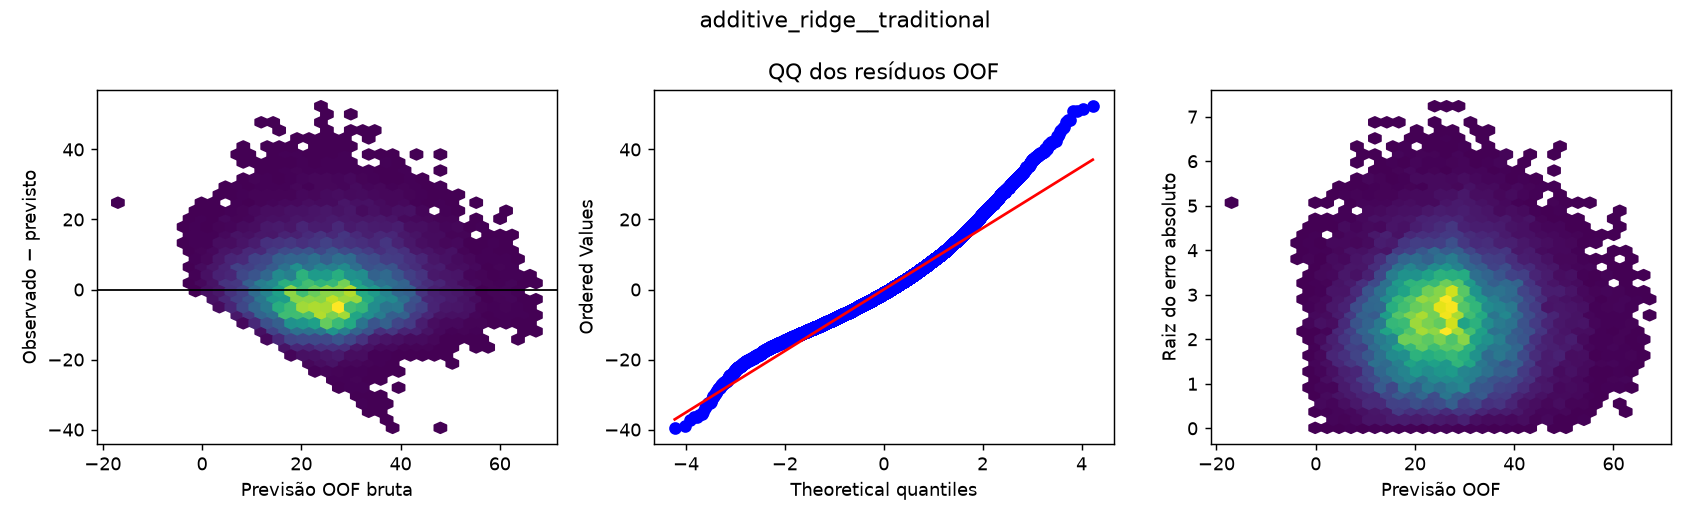
\includegraphics[width=\linewidth]{images/residuos_tradicional_aditivo.png}
\caption{Diagnósticos dos resíduos OOF da regressão aditiva com Ridge no bloco Tradicional}\label{fig:residuos}
\fonte{Execução da modelagem da coorte aceita. Figura original preservada.}
\nota{À esquerda, resíduos versus previsões; ao centro, gráfico QQ; à direita, raiz do erro absoluto versus previsões. A orientação horizontal permite ler os três painéis. Nenhuma previsão foi recalibrada para produzir esta figura.}
\end{figure}
\end{landscape}

\clearpage
\section{Discussão e alcance dos resultados}

A análise permitiu avaliar duas questões complementares. A primeira foi se as características disponíveis fornecem informação para estimar a popularidade observada. A redução do erro em relação às referências constantes indica que sim, dentro da coorte analisada. A segunda foi se os descritores de letras acrescentam informação ao Baseline. A comparação pareada mostrou melhora pequena, mas consistente, especialmente ao examinar a regressão aditiva com Ridge.

O resultado central pode ser sintetizado da seguinte forma: em 58.633 composições operacionais do desenvolvimento, avaliadas por validação cruzada agrupada e aninhada, o bloco Tradicional aditivo alcançou MAE de 6,8906, RMSE de 8,9016 e $R^2$ de 0,5612. Frente ao Baseline da mesma família, houve melhora das três métricas, redução do P95 do erro e diminuição agregada dos erros superiores a 20 pontos. A melhora do MAE foi inferior a um décimo de ponto e, por isso, deve ser descrita como contribuição incremental modesta.

A comparação não demonstra que propriedades das letras causem maior popularidade. Tampouco identifica uma propriedade textual específica como responsável pelo ganho: as 196 variáveis foram avaliadas como bloco, e muitas são correlacionadas. A investigação de efeitos individuais exigiria procedimentos próprios e cuidados adicionais com seleção de variáveis, dependência e interpretação de coeficientes.

A escassez de composições com resposta elevada é uma limitação relevante. Embora a amostra total seja numerosa, apenas 149 composições tinham popularidade de pelo menos 70, das quais 11 estavam entre 80 e 89. Esse desequilíbrio explica por que não se deve confundir precisão média com desempenho para grandes valores da resposta. A análise não permite decompor quanto do erro nessa região resulta de escassez amostral, atributos insuficientes, forma do modelo ou características não observadas.

Há outras limitações. A seleção por disponibilidade de letra modifica o perfil da base; a composição é definida operacionalmente; a auditoria de hashes exclui sobreposição textual exata entre splits, mas não substitui revisão humana do pareamento ou detecção de paráfrases e versões próximas. Além disso, os descritores LFM2b e os textos LRCLIB podem não representar exatamente a mesma versão da letra. Esses pontos restringem a generalização e devem permanecer explícitos na monografia.

As métricas não devem ser comparadas diretamente às de rodadas anteriores com menor amostra externa de validação, pois os denominadores e a composição dos conjuntos mudaram. Nesta rodada, as comparações internas são alinhadas: os blocos usam as mesmas observações e partições. O holdout originalmente avaliado na V0.6 não é uma nova confirmação independente, e seus alvos não foram carregados nesta etapa.

Do ponto de vista computacional, a execução completa durou aproximadamente 23 minutos e salvou 50 modelos de folds. As previsões foram reproduzidas com diferença numérica máxima igual a zero. Os arquivos de entrada permaneceram inalterados, e nenhuma configuração interna falhou. Foram registrados avisos de categorias não observadas no treino, tratados pela regra de codificação prevista. Essa verificação demonstra reprodutibilidade computacional dos artefatos; não comprova, por si só, ausência de todos os possíveis vieses científicos.

Por fim, esta etapa não utilizou embeddings na coorte ampliada. O bloco Tradicional já incorpora descritores de letras, mas a contribuição de representações produzidas por uma rede pré-treinada continua sendo uma pergunta a investigar. Uma etapa posterior deverá preservar a coorte e as partições, acrescentar essas representações e comparar os blocos Profundo e Combinado com as referências aqui estabelecidas. Até lá, não há evidência nesta rodada de que embeddings melhorem ou piorem o desempenho.

O principal avanço é, portanto, uma referência estatística reproduzível e interpretável: sabe-se quantas composições foram avaliadas, como os modelos foram selecionados, em quanto os descritores melhoraram as métricas e onde permaneceram as maiores dificuldades. Esses resultados delimitam o que foi alcançado e orientam a próxima comparação, sem antecipar suas conclusões.

\clearpage
\begin{thebibliography}{99}
\addcontentsline{toc}{section}{Referências}
\bibitem[Cawley e Talbot(2010)]{cawley2010}
CAWLEY, Gavin C.; TALBOT, Nicola L. C. On over-fitting in model selection and subsequent selection bias in performance evaluation. \textit{Journal of Machine Learning Research}, v. 11, p. 2079--2107, 2010. Disponível em: \url{https://www.jmlr.org/papers/v11/cawley10a.html}.
\bibitem[James et al.(2023)]{james2023}
JAMES, Gareth; WITTEN, Daniela; HASTIE, Trevor; TIBSHIRANI, Robert; TAYLOR, Jonathan. \textit{An Introduction to Statistical Learning with Applications in Python}. Cham: Springer, 2023. Material dos autores disponível em: \url{https://www.statlearning.com/}.
\end{thebibliography}

\end{document}
